% \providecommand{\main}{..} 

\documentclass[../main.tex]{subfiles}
\graphicspath{{\subfix{../figures/}}}
\usepackage{bbm}

% \addbibresource{../bibliography/bibliography.bib} % 

\begin{document}
\chapter{Introduction}
\label{chap:intro}

	% COMENZAR A ESCRIBIR EL TRABAJO
	% \section{Background} \label{background}
% @ts-ignore
 As health information becomes increasingly digitized, machine learning (ML) algorithms play a crucial role in deriving meaningful insights from complex, multi-modal data that is often difficult to interpret by humans. 
 Conventional machine-learning approaches, however, may be inadequate in the face of rapidly evolving health technology, shifting patient needs, and the increasing availability of large amounts of uncertain and noisy data that is deemed too unreliable for use in clinical settings.

 Modern techniques aim to address these limitations by refining models in a continual loop, prioritizing data acquisition, labeling, and feedback from experts to dynamically adapt to the data stream reliably. This work explores the potential of these techniques in the context of healthcare applications.
 
 In particular, we incorporate the use of continual and active learning methods in the design of an end-to-end platform for the diagnosis of \textit{tuberculosis} using computer vision techniques. Tuberculosis (TB) is an infectious pulmonary disease that has affected humankind for well over 4,000 years \cite{cdctb_world_2023} and still affects millions of people worldwide. According to the World Health Organization, until the arrival of the COVID-19 pandemic, TB was the leading cause of widespread death from a single infectious agent, ranking even above HIV/AIDS \cite{who_global_2022}.

 The platform is meant to be integrated into a Healthcare and Data Portal that is being developed as part of an ongoing European project for the research of Tuberculosis, and it will serve as a tool to test and validate the use of machine-learning models for the diagnosis of Tuberculosis. 

 As such, in an effort to research the competence of continual adaptation methods in that context, the platform incorporates a system that is designed to continually adapt to new data as it becomes available and to ease labeling efforts by prioritizing the acquisition of the most informative data samples. Including a front-end interface for the visualization of the detection, labeling, and interaction with the models.
 
 We evaluate the system's performance on a real dataset and compare it to a baseline model that doesn't use adaptation techniques.  Our results show that the use of these methods outperforms the baseline in terms of robustness and sample efficiency while maintaining a similar level of accuracy on the test set. Furthermore, the system proposed can automatically adapt to new data and improve its performance over time. 
 
 These results demonstrate the potential of incorporating these techniques into designing real-world systems for healthcare applications and other high-stake domains. The final chapter of this work includes a lengthy discussion about possible future work and improvements to the system that might facilitate its integration into other projects and applications.
    
 \section{Context and Motivation} \label{sec:motivation}
%  \section{An ML Platform to aid on the research of Mycobacterial Tuberculosis (TB)}
%  drug discovery and early detection of

    This work is done in the context of the European Regimen Accelerator for Tuberculosis (ERA4TB). ERA4TB is a public-private initiative that started in 2020 and aims to create an open European platform to accelerate the development of new treatment regimens for tuberculosis (TB). The project is integrated by over 31 organizations from the European Union and the United States, including academic institutions, research centers, non-profit organizations, and other public and private entities \cite{noauthor_era4tb}.
    
    ERA4TB's mission statement aligns itself with (and is in response to) the United Nation's (UN) Sustainable Development Goals (SGD). The project's website reads, `The goal of ERA4TB is to deliver an innovative and differentiated combination regimen for the treatment of TB, which can play a key role in the TB elimination agenda' \cite{noauthor_era4tb}. This aligns with the UN's SGD target to end the TB epidemic by 2030 \cite{world_health_organization_regional_office_for_europe_tuberculosis_2017}.

    To address some of the challenges of TB drug development and clinical trial design, one of the project's objectives from deliverable 1.15 of ERA4TB's agenda is developing a data-science-specific platform to enable the efficient use of machine learning methods from the collaborative platform. The platform is meant to be used by researchers and other project stakeholders to facilitate the use, development, and evaluation of machine-learning models that can aid in the research of TB.

    Thus, the motivation behind this work comes from the idea of incorporating novel methods into this data-science-specific platform to support researchers and collaborators in their mission to end TB by 2030. The techniques described in this work are designed to improve the performance of supervised models while prioritizing their overall robustness and reliability, aspects that are crucial in the context of healthcare applications.

    \begin{figure}[H]
        \centering
        \includegraphics[width=\textwidth]{figures/ERA4TB_map.png}
        \caption{ERA4TB's Consortium of Partners and Collaborators. Source: \cite{noauthor_era4tb}}
        \label{fig:era4tb}
    \end{figure}

    \section{Background Concepts} \label{sec:background}
    
    The following section provides a brief introduction to some of the concepts and techniques that are relevant to this work. It is meant to provide the reader with the necessary high-level information to understand the context and motivation behind the ideas proposed that were used to inform every design decision and experiment conducted. For a more in-depth overview of the same concepts, the reader is referred to the literature review in Chapter \ref{chap:state_of_the_art}.

    \subsection{Tuberculosis Treatment and Diagnosis} \label{sec:tuberculosis_data}

    Tuberculosis is caused by the bacillus (bacteria) \textit{Mycobacterium tuberculosis} (MTB), which is transmitted when people who are sick with TB expel the bacteria into the air by coughing, sneezing, or spitting. The disease is preventable with the administration of a vaccine and curable with the use of antibiotics over a significant period (although drug-resistant strains of the bacteria are becoming increasingly common) \cite{who_tuberculosis_2023}.
    
    Nonetheless, the disease is often underdiagnosed and undertreated, especially in low-resource settings (i.e., developing countries, rural areas, and marginalized/impoverished communities), where the disease is more prevalent, calling for the development of more efficient and cost-effective methodologies to diagnose and treat the disease \cite{who_global_2022, imi_era4tb_2020,  who_tuberculosis_2023}.

    Some of the diagnosis techniques to detect TB include chest X-rays, sputum smear microscopy, and molecular tests. \textit{Chest X-rays} are a common procedure to diagnose any signs of tuberculosis due to the wide availability of radiology devices, but they are often inconclusive and require expert radiologists to interpret the results \cite{escalante_tuberculosis_2009}.
    
    \textit{Sputum smear microscopy} is another widely available technique that requires a trained clinician to identify the bacteria under images taken with a microscope of a patient's sputum (a mixture of saliva and mucus from the respiratory tract). This technique is relatively inexpensive but requires a high concentration of bacteria in the sample to be effective. Additionally, studies argue that in conditions with limited resources and a significant number of samples, there have been reports of poor sample observation and quality control measures, which can result in false-negative results \cite{desikan_sputum_2013}.
    
    Molecular tests based on \textit{nucleic acid amplification} (NAATs), similar to the ones popularized to detect COVID-19, are another technique to diagnose TB. These tests identify the presence of bacilli by amplifying the genetic material of the bacteria in a patient's sputum sample (if any is present) and using a chemical solution to react to it \cite{cdc_tb_2016}. NAATs are by far the most reliable method to diagnose TB and have the advantage of being rapid and fully automated. 
    
    However, NAATs are expensive to produce and require specialized equipment, making them less accessible in low-resource settings \cite{albert_development_2016, maclean_advances_2020}. Indeed, a study conducted in 2018 showed that the ratio of smear microscopy tests to NAATs in countries with a high burden of TB was 6:1 \cite{cazabon_market_2018, maclean_advances_2020}.

    Each of these techniques presents its own benefits and limitations. Recently, there have been efforts to develop machine-learning models that can aid in the diagnosis of TB as a way to reduce the need (or provide a first/second opinion) for expert clinicians in the process and improve the speed and/or accuracy of the diagnosis \footnote{A literature review on the topic of TB diagnosis using ML methods is presented in section \ref{sec:ml_tuberculosis_detection}}.

    \begin{figure}
        \begin{subfigure}{130px}
          \centering
        %   \frame{
            \includegraphics[width=120px,height=120px]{chest_x_ray.png}
        %   }
        %   \caption{Chest X-Ray }
          \label{fig:chest_x_ray_example}
        \end{subfigure}%
        \begin{subfigure}{130px}
          \centering
        %   \frame{
          \includegraphics[width=120px,height=120px]{sputum_smear.png}
        %   }
        %   \caption{Sputum Smear with Tuberculosis Bacilli}
          \label{fig:sputum_smear_exmaple}
        \end{subfigure}
        \begin{subfigure}{130px}
          \centering
        %   \frame{
          \includegraphics[width=120px,height=120px]{MTB_RIF_Test.jpeg}
        %   }
        %   \caption{Example of Procedure of a Molecular Test for MTB}
          \label{fig:molecular_test_example}
        \end{subfigure}
        \caption{
            Examples of common techniques to diagnose Tuberculosis.
            Left: Chest X-ray of a patient with TB \cite{ubaidi_radiological_nodate}. Middle: Sputum smear with tuberculosis bacilli \cite{shah_ziehlneelsen_2017}. Right: Example of a molecular test for MTB \cite{boehme_rapid_2010}.
        }
        \label{fig:tuberculosis_diagnosis_examples}
    \end{figure}
    
    \subsection{Supervised and Semi-Supervised Machine-Learning} \label{sec:supervised_ml}

    Machine Learning (ML) is a subfield of Artificial Intelligence (AI) that studies the design of algorithms that can learn from data and make predictions based on it. ML algorithms are fed a set of data samples (often called the training set) and learn a function that maps the input data to a desired output. The goal is to learn a function that can generalize well to unseen data and make accurate predictions. 

    Supervised learning is a paradigm of ML where the goal is to fit a function $f: x \rightarrow \hat{y}$ that maps a given input, $x$, to a `prediction' output, $\hat{y}$, based on an available finite set of input-output pairs $(x_i, y_i)$ that are passed to a learnable model as `training' data. The function is learned by minimizing a loss function $L(y, \hat{y})$ that measures the difference between the `predicted' output and the actual one and returns a value that represents the error of the prediction, which is then used to update the model's parameters.

    The most common supervised learning tasks are classification and regression, where the goal is to predict discrete and continuous outputs, respectively. Conversely, the aforementioned loss function is often defined based on the task at hand and the type of data available (e.g., cross-entropy loss for classification tasks, mean squared error for regression tasks, etc.).

    The presence of a known output (or label) for each input is what makes this paradigm `supervised'. For example, in healthcare, supervised learning might be used to predict the presence of a disease or condition based on a set of features extracted (or learned) from the patient's data. A model can be trained to predict the presence or severity of a disease based on a set of symptoms, clinical history, or imaging data.

    Besides its many benefits, the most significant disadvantage of supervised learning is that it often needs large amounts of labeled samples to produce accurate and robust results \cite{lecun_deep_2015}, 
    approaches such as \textit{semi-supervised learning} (sometimes also called weak supervision) aim to address this issue by leveraging both labeled and unlabeled data to train the model \cite{zhu_semi-supervised_2008}. 
    
    Semi-supervised learning works by using unlabeled samples to learn an intermediary representation of the data that can be used as a first step to train a supervised model. This approach is especially useful when the unlabeled data is abundant and easy to obtain, but their labels are scarce and expensive. This is often the case in some healthcare applications, where the labeling task can only be performed by professional workers, making it a costly and time-consuming task \cite{yakimovich_labels_2021,chen_study_2015, figueroa_predicting_2012}.
    
    % which is especially challenging in the healthcare field where the data is scarce, expensive to obtain, or difficult to label.
    
    \begin{figure}
        \centering
        \resizebox*{1\columnwidth}{!}{
            % \hspace*{-0.5cm}
            \tikzset{every picture/.style={line width=0.2pt}} %set default line width to 0.75pt        


\begin{tikzpicture}[x=0.75pt,y=0.75pt,yscale=-1,xscale=1]
%uncomment if require: 
\path (0,446); %set diagram left start at 0, and has height of 446
%Shape: Rectangle [id:dp03411876837432981] 
\draw[fill={rgb, 255:red, 30; green, 164; blue, 247 }  ,fill opacity=0.36 ] (13,71.03) -- (225.26,71.03) -- (225.26,244.73) -- (13,244.73) -- cycle ;
%Shape: Triangle [id:dp9375754488130867] 
\draw  [fill={rgb, 255:red, 208; green, 2; blue, 27 }  ,fill opacity=1 ] (126.3,85.43) -- (147.81,120.93) -- (104.79,120.93) -- cycle ;
%Shape: Ellipse [id:dp16442697541796703] 
\draw  [fill={rgb, 255:red, 74; green, 144; blue, 226 }  ,fill opacity=1 ] (133.47,153.08) .. controls (133.47,142.22) and (142.25,133.41) .. (153.07,133.41) .. controls (163.9,133.41) and (172.67,142.22) .. (172.67,153.08) .. controls (172.67,163.95) and (163.9,172.76) .. (153.07,172.76) .. controls (142.25,172.76) and (133.47,163.95) .. (133.47,153.08) -- cycle ;
%Shape: Ellipse [id:dp8929359456575365] 
\draw  [fill={rgb, 255:red, 74; green, 144; blue, 226 }  ,fill opacity=1 ] (23.52,153.08) .. controls (23.52,142.22) and (32.29,133.41) .. (43.12,133.41) .. controls (53.94,133.41) and (62.72,142.22) .. (62.72,153.08) .. controls (62.72,163.95) and (53.94,172.76) .. (43.12,172.76) .. controls (32.29,172.76) and (23.52,163.95) .. (23.52,153.08) -- cycle ;
%Shape: Triangle [id:dp7376655464767954] 
\draw  [fill={rgb, 255:red, 208; green, 2; blue, 27 }  ,fill opacity=1 ] (61.28,85.43) -- (82.8,120.93) -- (39.77,120.93) -- cycle ;
%Shape: Rectangle [id:dp12169534238909918] 
\draw  [fill={rgb, 255:red, 245; green, 166; blue, 35 }  ,fill opacity=1 ] (160.24,88.31) -- (199.44,88.31) -- (199.44,127.65) -- (160.24,127.65) -- cycle ;
%Shape: Rectangle [id:dp008860357027288712] 
\draw  [fill={rgb, 255:red, 245; green, 166; blue, 35 }  ,fill opacity=1 ] (165.02,184.27) -- (204.22,184.27) -- (204.22,223.62) -- (165.02,223.62) -- cycle ;
%Shape: Rectangle [id:dp9615704991146319] 
\draw  [fill={rgb, 255:red, 245; green, 166; blue, 35 }  ,fill opacity=1 ] (77.54,134.37) -- (116.74,134.37) -- (116.74,173.72) -- (77.54,173.72) -- cycle ;
%Shape: Triangle [id:dp3026521490627023] 
\draw  [fill={rgb, 255:red, 208; green, 2; blue, 27 }  ,fill opacity=1 ] (124.39,184.27) -- (145.9,219.78) -- (102.88,219.78) -- cycle ;
%Shape: Ellipse [id:dp47582021898019566] 
\draw  [fill={rgb, 255:red, 74; green, 144; blue, 226 }  ,fill opacity=1 ] (39.77,204.91) .. controls (39.77,194.04) and (48.55,185.23) .. (59.37,185.23) .. controls (70.2,185.23) and (78.97,194.04) .. (78.97,204.91) .. controls (78.97,215.77) and (70.2,224.58) .. (59.37,224.58) .. controls (48.55,224.58) and (39.77,215.77) .. (39.77,204.91) -- cycle ;
%Shape: Rectangle [id:dp29141062253976635] 
\draw  [fill={rgb, 255:red, 247; green, 204; blue, 30 }  ,fill opacity=0.36 ] (14.91,278.32) -- (227.17,278.32) -- (227.17,374.29) -- (14.91,374.29) -- cycle ;
%Shape: Ellipse [id:dp4851406617475926] 
\draw  [fill={rgb, 255:red, 74; green, 144; blue, 226 }  ,fill opacity=1 ] (100.96,312.39) .. controls (100.96,301.52) and (109.74,292.72) .. (120.56,292.72) .. controls (131.39,292.72) and (140.16,301.52) .. (140.16,312.39) .. controls (140.16,323.25) and (131.39,332.06) .. (120.56,332.06) .. controls (109.74,332.06) and (100.96,323.25) .. (100.96,312.39) -- cycle ;
%Shape: Triangle [id:dp1307613946933155] 
\draw  [fill={rgb, 255:red, 208; green, 2; blue, 27 }  ,fill opacity=1 ] (64.15,292.72) -- (85.66,328.22) -- (42.64,328.22) -- cycle ;
%Shape: Rectangle [id:dp35663833636935394] 
\draw  [fill={rgb, 255:red, 245; green, 166; blue, 35 }  ,fill opacity=1 ] (165.98,293.67) -- (205.18,293.67) -- (205.18,333.02) -- (165.98,333.02) -- cycle ;
%Straight Lines [id:da6673185348400361] 
\draw    (263.82,213.55) -- (298.82,213.5) ;
\draw [shift={(300.82,213.49)}, rotate = 179.91] [color={rgb, 255:red, 0; green, 0; blue, 0 }  ][line width=0.75]    (10.93,-3.29) .. controls (6.95,-1.4) and (3.31,-0.3) .. (0,0) .. controls (3.31,0.3) and (6.95,1.4) .. (10.93,3.29)   ;
%Straight Lines [id:da17452505371177662] 
\draw    (227,322.73) -- (263.54,323.73) ;
%Straight Lines [id:da19470043848262208] 
\draw    (226.21,149.72) -- (264.67,150.72) ;
%Straight Lines [id:da10397627231220286] 
\draw    (264.67,150.72) -- (263.54,323.73) ;
%Shape: Ellipse [id:dp8385531363983802] 
\draw  [fill={rgb, 255:red, 80; green, 227; blue, 194 }  ,fill opacity=0.49 ][dash pattern={on 4.5pt off 4.5pt}] (300.82,213.49) .. controls (300.82,180.48) and (341.79,153.71) .. (392.32,153.71) .. controls (442.86,153.71) and (483.82,180.48) .. (483.82,213.49) .. controls (483.82,246.51) and (442.86,273.28) .. (392.32,273.28) .. controls (341.79,273.28) and (300.82,246.51) .. (300.82,213.49) -- cycle ;
%Straight Lines [id:da2475999051951534] 
\draw    (483.82,213.49) -- (526.82,213.29) ;
\draw [shift={(528.82,213.28)}, rotate = 179.73] [color={rgb, 255:red, 0; green, 0; blue, 0 }  ][line width=0.75]    (10.93,-3.29) .. controls (6.95,-1.4) and (3.31,-0.3) .. (0,0) .. controls (3.31,0.3) and (6.95,1.4) .. (10.93,3.29)   ;
%Shape: Rectangle [id:dp03611177475200367] 
\draw  [fill={rgb, 255:red, 30; green, 164; blue, 247 }  ,fill opacity=0.36 ] (493.91,313.59) -- (664.82,313.59) -- (664.82,376.82) -- (493.91,376.82) -- cycle ;
%Shape: Triangle [id:dp8126894821695971] 
\draw  [fill={rgb, 255:red, 208; green, 2; blue, 27 }  ,fill opacity=1 ] (514.8,330.86) -- (530.82,360.28) -- (498.77,360.28) -- cycle ;
%Shape: Rectangle [id:dp7704102629126468] 
\draw  [fill={rgb, 255:red, 245; green, 166; blue, 35 }  ,fill opacity=1 ] (587.24,330.74) -- (611.82,330.74) -- (611.82,357.28) -- (587.24,357.28) -- cycle ;
%Shape: Ellipse [id:dp8221231723533802] 
\draw  [fill={rgb, 255:red, 74; green, 144; blue, 226 }  ,fill opacity=1 ] (540.96,346) .. controls (540.96,337) and (548.32,329.72) .. (557.39,329.72) .. controls (566.47,329.72) and (573.82,337) .. (573.82,346) .. controls (573.82,354.99) and (566.47,362.28) .. (557.39,362.28) .. controls (548.32,362.28) and (540.96,354.99) .. (540.96,346) -- cycle ;
%Shape: Ellipse [id:dp6362055661503672] 
\draw  [fill={rgb, 255:red, 74; green, 144; blue, 226 }  ,fill opacity=1 ] (622.82,343.78) .. controls (622.82,335.22) and (629.54,328.28) .. (637.82,328.28) .. controls (646.11,328.28) and (652.82,335.22) .. (652.82,343.78) .. controls (652.82,352.34) and (646.11,359.28) .. (637.82,359.28) .. controls (629.54,359.28) and (622.82,352.34) .. (622.82,343.78) -- cycle ;
%Rounded Rect [id:dp4276999307253777] 
\draw  [fill={rgb, 255:red, 189; green, 16; blue, 224 }  ,fill opacity=0.24 ][dash pattern={on 4.5pt off 4.5pt}] (530,191.88) .. controls (530,183.26) and (536.98,176.28) .. (545.6,176.28) -- (612.22,176.28) .. controls (620.84,176.28) and (627.82,183.26) .. (627.82,191.88) -- (627.82,238.68) .. controls (627.82,247.29) and (620.84,254.28) .. (612.22,254.28) -- (545.6,254.28) .. controls (536.98,254.28) and (530,247.29) .. (530,238.68) -- cycle ;
%Straight Lines [id:da16188474121366347] 
\draw    (580,314) -- (580.79,256.19) ;
\draw [shift={(580.82,254.19)}, rotate = 90.79] [color={rgb, 255:red, 0; green, 0; blue, 0 }  ][line width=0.75]    (10.93,-3.29) .. controls (6.95,-1.4) and (3.31,-0.3) .. (0,0) .. controls (3.31,0.3) and (6.95,1.4) .. (10.93,3.29)   ;
%Straight Lines [id:da6849788730551594] 
\draw    (628.41,211.78) -- (667.82,211.82) ;
\draw [shift={(669.82,211.82)}, rotate = 180.05] [color={rgb, 255:red, 0; green, 0; blue, 0 }  ][line width=0.75]    (10.93,-3.29) .. controls (6.95,-1.4) and (3.31,-0.3) .. (0,0) .. controls (3.31,0.3) and (6.95,1.4) .. (10.93,3.29)   ;
%Shape: Cube [id:dp11030403935801325] 
\draw  [fill={rgb, 255:red, 155; green, 155; blue, 155 }  ,fill opacity=1 ] (669,192.65) -- (688.01,173.64) -- (735.82,173.64) -- (735.82,217.99) -- (716.81,237) -- (669,237) -- cycle ; \draw   (735.82,173.64) -- (716.81,192.65) -- (669,192.65) ; \draw   (716.81,192.65) -- (716.81,237) ;
%Shape: Triangle [id:dp48891639752656224] 
\draw  [fill={rgb, 255:red, 208; green, 2; blue, 27 }  ,fill opacity=0.74 ] (693.82,204.64) -- (704.82,223.28) -- (682.77,223.28) -- cycle ;
%Shape: Ellipse [id:dp8314174152258622] 
\draw  [fill={rgb, 255:red, 74; green, 144; blue, 226 }  ,fill opacity=0.61 ] (692.68,182.96) .. controls (695.97,179.47) and (703.99,176.64) .. (710.59,176.64) .. controls (717.19,176.64) and (719.86,179.47) .. (716.57,182.96) .. controls (713.27,186.45) and (705.25,189.28) .. (698.66,189.28) .. controls (692.06,189.28) and (689.38,186.45) .. (692.68,182.96) -- cycle ;
%Shape: Rectangle [id:dp03254240217615467] 
\draw  [fill={rgb, 255:red, 245; green, 166; blue, 35 }  ,fill opacity=0.55 ] (720.08,200.39) -- (732.82,188.28) -- (732.38,210.57) -- (719.65,222.67) -- cycle ;

% Text Node
\draw (291,9) node [anchor=north west][inner sep=0.75pt]   [align=left] {{\fontfamily{helvet}\selectfont {\Large Supervised Learning}}};
% Text Node
\draw (74.98,48.58) node [anchor=north west][inner sep=0.75pt]   [align=left] {Training Data};
% Text Node
\draw (92.3,379.7) node [anchor=north west][inner sep=0.75pt]   [align=left] {Labels};
% Text Node
\draw (40.7,341.4) node [anchor=north west][inner sep=0.75pt]  [font=\footnotesize] [align=left] {Triangle};
% Text Node
\draw (100.26,340.44) node [anchor=north west][inner sep=0.75pt]  [font=\footnotesize] [align=left] {Circle};
% Text Node
\draw (165.08,341.4) node [anchor=north west][inner sep=0.75pt]  [font=\footnotesize] [align=left] {Square};
% Text Node
\draw (330,177.4) node [anchor=north west][inner sep=0.75pt]    {$ \begin{array}{l}
\ \ \ \ \ f_{i}(\textcolor[rgb]{0.82,0.01,0.11}{\blacktriangle }) =\ \hat{y}\\
\mathcal{L}( y,\ \hat{y}) \ \rightarrow f_{i+1} \ 
\end{array}$};
% Text Node
\draw (312,123) node [anchor=north west][inner sep=0.75pt]   [align=left] {{\Large \faCog}};
% Text Node
\draw (341.98,125.58) node [anchor=north west][inner sep=0.75pt]   [align=left] {Model Training};
% Text Node
\draw (449,122) node [anchor=north west][inner sep=0.75pt]   [align=left] {{\Large \faCog}};
% Text Node
\draw (340,235) node [anchor=north west][inner sep=0.75pt]   [align=left] {{\footnotesize Learning algorithm}};
% Text Node
\draw (551.98,386.01) node [anchor=north west][inner sep=0.75pt]   [align=left] {Test Data};
% Text Node
\draw (520,132) node [anchor=north west][inner sep=0.75pt]   [align=left] {\begin{minipage}[lt]{86.41pt}\setlength\topsep{0pt}
\begin{center}
{\small Model }\\{\small Inference/Evaluation}
\end{center}

\end{minipage}};
% Text Node
\draw (533,193) node [anchor=north west][inner sep=0.75pt]   [align=left] {$\displaystyle f(\textcolor[rgb]{0.82,0.01,0.11}{\blacktriangle })$};
% Text Node
\draw (572,194) node [anchor=north west][inner sep=0.75pt]   [align=left] {{\scriptsize = Triangle?}};
% Text Node
\draw (543.82,220.28) node [anchor=north west][inner sep=0.75pt]   [align=left] {{\scriptsize \textcolor[rgb]{0.29,0.29,0.29}{metric = 0.999 }}};
% Text Node
\draw (668.98,152.01) node [anchor=north west][inner sep=0.75pt]   [align=left] {Final Model};
% Text Node
\draw (653,249) node [anchor=north west][inner sep=0.75pt]   [align=left] {$\displaystyle f(\textcolor[rgb]{0.82,0.01,0.11}{\blacktriangle ,}\textcolor[rgb]{0.29,0.56,0.89}{\bullet} ,\textcolor[rgb]{0.96,0.65,0.14}{\blacksquare }) \tiny{=\{label\}}$  };

\end{tikzpicture}


        }
        \caption{Illustrative example of a supervised machine-learning pipeline.}
        \label{fig:supervised_learning}
    \end{figure}
    
    In the two decades, one set of algorithms that have enabled significant advances in Machine Learning, allowing to solve very difficult problems, is \textbf{deep learning}. Deep learning is a subfield of ML that studies the design of algorithms that can learn complex representations of data by hierarchically composing simpler functions in an architecture inspired by the structure of the human brain known as `Deep Neural Networks' (DNN)  \cite{lecun_deep_2015}. Figure \ref{fig:dnn_example} shows an example of a DNN architecture.
    
    \begin{figure}[H]
        \centering
        \resizebox*{0.5\columnwidth}{!}{
            % \hspace*{-0.5cm}
            \includegraphics{dnn_example_topol}
        }
        \caption{Example of a simplified neural network architecture taken from \cite{topol_high-performance_2019}.}
        \label{fig:dnn_example}
    \end{figure}

    \clearpage
    \subsection{Challenges and Potential of Adopting ML-enabled Systems in Healthcare}

    ML techniques have seen their adoption in many applications, from malware and spam detection to self-driving cars and environmental modeling. The healthcare field is no exception. In the 20 years between 1995 and 2015, the FDA had approved fewer than 30 algorithms for medical use. In contrast, only in the last 5 years, the number of new approvals has reached over \textit{10 times} that amount (see Figure \ref{fig:fda_approved_ml_apps}). 
    
    Indeed, the recent availability to store and process ever larger amounts of data through the use of Big Data technologies and the development of more powerful hardware and algorithmic techniques have made it possible to train models that can perform complex medical tasks with enough high accuracy and robustness to be considered for use
    \cite{topol_high-performance_2019}.

    Of such techniques, some that have recently disrupted the medical field are those based on \textbf{computer vision}  (CV). CV methods try to develop algorithms that enable computers to solve visual tasks. It is a broad field that has been applied to problems like image classification, object detection, and image segmentation and has seen significant advances in the last decade thanks to the adoption of Deep Learning algorithms \cite{lecun_deep_2015}.

    In the context of healthcare, CV techniques have been primarily used in radiology to aid with the diagnosis of diseases and other tasks through the analysis of medical images (e.g., X-rays, CT scans, MRIs, microscopy, etc.) \cite{esteva_deep_2021}. Indeed, over 75\% of all FDA-cleared AI applications have been for radiology use cases \cite{health_artificial_2022}.
    
    One study made in 2018 trained a \textit{Convolutional Neural Network} (CNN), a common DL model popular for computer vision tasks, to detect pneumonia from X-ray images at an Indian hospital. The researchers compared the performance of the algorithm with the findings of four expert radiologists and concluded that the algorithm was comparable to (sometimes even \textit{outperformed}) the radiologist in most cases \cite{wang_chestx-ray8_2017}.
    
    \begin{figure}[H]
        \centering
        \includegraphics[width=0.9\textwidth]{fda_approved_ml_apps}
        \caption{Number of FDA-approved AI applications per year since 2005. Data Source: \cite{health_artificial_2022}}
        \label{fig:fda_approved_ml_apps}
    \end{figure}

    Other AI systems such as Google Deepmind's \textit{AlphaFold} \cite{yang_alphafold2_2023} have been shown to predict the 3D structure of proteins with high accuracy, solving a problem that had been considered to be one of the most challenging in computational biology for over 50 years. Such breakthrough is thought to have a significant impact in applications like drug discovery in the near future \cite{jumper_highly_2021}.
    
    Results such as these shine a light on the potential that AI techniques have in the medical field. However, the adoption of such technologies doesn't come with new challenges. Experts have emphasized the importance of improving aspects of these models like their lack of interpretability, robustness to unseen data, and the difficulty of integrating them into existing workflows before they can be widely adopted in clinical settings \cite{esteva_deep_2021, topol_high-performance_2019}.
    
    Thus, the design of ml-enabled systems must be mindful of the limitations of such models. Research in the healthcare and AI fields must pave the way to develop workflows that can be trusted by clinicians, patients, lawmakers, and other researchers alike to improve the quality of care/research, reduce costs, and overall increase the efficiency of the healthcare system.

     \begin{table}[h]
        \resizebox{0.9\textwidth}{!}{
            \begin{tabular}{lrll}
                \toprule
                Company &  Year & Usecase & Panel \\
                \midrule
                Apple &  2022 & Atrial Fibrillation Detection via Apple Watch & Cardiovascular \\
                Arterys &  2022 & Liver and Lung Cancer Detection & Radiology \\
                Philips Healthcare &  2022 & Philips Incisive CT Reconstruction & Radiology \\ 
                GE Healthcare &  2021 & Deep Learning Image Reconstruction &  Radiology \\
                Siemens &  2021 & AI-Rad Companion for CT Interpretation & Radiology \\
                Icometrix &  2018 & Brain MRI Analysis & Radiology \\ 
                23\&Me &  2017 & Genetic Testing for Hereditary Thrombophilia & Hematology \\
                \bottomrule
            \end{tabular}
            \caption{Examples of FDA-approved AI applications for medical use. S\lowercase{ource: \cite{health_artificial_2022}}}
        }
    \end{table}

    \subsection{Continually Adaptive Systems} \label{sec:continually_adaptive_systems}

    Table \ref{tab:causes_of_ml_degradation} lists some of the most common causes of degradation of a learning system and the techniques that can be used to address them. The causes and descriptions in the table were sourced from Casmiro et al.'s work on self-adaptive machine-learning \cite{casimiro_self-adaptive_2022} and Chip Huyen's book about Machine-Learning systems \cite{huyen_designing_2022} \cite{casimiro_self-adaptive_2022}.

    \begin{table}[h]
        \caption{Some Causes of Degradation of an ML System}
        \label{tab:causes_of_ml_degradation}
        \hspace*{-0.7cm}
        \begin{tabular}{p{0.25\linewidth} | p{0.45\linewidth} | p{0.35\linewidth}}
        \toprule
        \textbf{Cause} & \textbf{Description} & \textbf{Example} \\
        \midrule
            \multirow{3}{*}{\small \textbf{Data distribution shift}} & \footnotesize
            \textbf{Covariate shift:} When the input distribution $P(X)$ that the model was trained with differs significantly from the one in the inference environment (i.e. the input changes over time, but the model remains the same). &
            \footnotesize
            A model trained on chest X-ray images from a particular dataset is deployed in a hospital where the X-ray machines are of a different brand and produce images with different characteristics.
            \\
            \cline{2-3} & \footnotesize
            \textbf{Label shift:} When the distribution  $P(Y)$ at inference time differs from the one the model was trained with, i.e. the model is trained on a dataset whose class proportions are substantially different from the ones in the inference environment. &
            \footnotesize
            A model trained on a dataset where the proportion of positive cases is 50\% is deployed in a hospital where the proportion is 10\%.
            \footnotesize
            \\
            \cline{2-3} & \footnotesize
            \textbf{Concept shift:} \footnotesize The relationship between the input and output changes over time. That is, the model is trained on a dataset whose relationship between the input and output differs from the one in the inference environment. &  \\
        \midrule
        \multirow{2}{*}{\small \textbf{Model}} & \footnotesize
            \textbf{Model drift:}The model's performance degrades over time. 
                & ? \\
            \cline{2-3} & \footnotesize
            \textbf{Model bias:} The model is biased towards a specific class or group. & \\
            \midrule
        \textbf{\small Environment drift} & \footnotesize 
            The environment changes over time. The model is deployed in a different environment than the one it was trained on.  & \\
        \bottomrule
        \end{tabular}
    \end{table}

    \todo[inline]{Add a brief description of the concept of continual adaptation and its relevance in the context of this work.}

    \clearpage

    \section{Objectives} \label{sec:objectives}

    \subsection*{Main objective} \label{sec:main_goal}

    The main objective of this work is to research the most relevant techniques on continual adaptation methods in Machine Learning, make a comparative analysis of the most relevant techniques and their relevance for health applications, and design and implement a system for the diagnosis of tuberculosis that incorporates these techniques into its design that can be integrated into the ERA4TB platform. The platform should allow its users to incorporate test machine-learning models into the platform and facilitate the use and collaboration between researchers and other stakeholders.

    \subsection*{Specific objectives} \label{sec:specific_objectives}

    Auxiliary to the main objective, the following specific objectives have been defined to guide the development of the work and evaluate its success:

    \begin{enumerate}
        \item The system should be capable of automatically triggering the continual learning process when new data is available or when the model's performance degrades based on a predefined metric.
        \item The platform must implement a feedback loop between the data annotation process and model training that prioritizes the acquisition of the most informative data samples to improve the model's performance (Active Learning).
        \item Develop a front-end interface that allows users to interact with the machine-learning models by selecting or submitting new data samples and visualizing the model's predictions.
        \item Consider the limitations of the proposed system and the ethical implications of its use and present a well-founded outline of necessary future work to address these limitations or improve the system in a way that aligns with the project's mission statement.
        \item Evaluate possible future research directions that could be explored in the area of continual and dynamic adaptation in Machine Learning, highlighting the contributions that have a higher potential for impact in healthcare or other high-stake domains.
    \end{enumerate}

    \clearpage

    \section{Main Contributions} \label{sec:main_contributions}

    \section{Structure of the Work} \label{sec:structure_of_the_work}

    This work is divided into five chapters, including this introduction. Chapter \ref{chap:intro} describes the context and motivation of this work and its objectives and provides the necessary background information to understand the concepts and techniques used. 
    
    Chapter \ref{chap:state_of_the_art} describes relevant work and state-of-the-art techniques. It also provides a literature review of related work in the field of machine learning methods for continual systems and their applications, highlighting the most important contributions and their limitations.

    Chapter \ref{chap:methodology} describes the methodology used to design and implement the proposed system.  It gives a detailed description of the data, models, techniques, and specific tools used in the implementation of the platform, experiments conducted, and relevant metrics to evaluate the system's performance.
    
    Chapter \ref{chap:results} presents the results of the experiments, analyzes the performance of the system, and compares the results with the baseline metrics. Finally, Chapter \ref{chap:conclusions} presents the conclusions and future work. It also discusses the limitations of the proposed system and the implications of the results obtained in the context of the project.

    
    

% \dobib
\end{document}